\documentclass[aip,jcp,reprint,showkeys]{revtex4-1}

\usepackage{graphicx,bm,xcolor,hyperref,amsmath,amssymb,amsfonts,float}



\newcommand{\alert}[1]{\textcolor{red}{#1}}
\newcommand{\ket}[1]{|#1\rangle}
\newcommand{\stwo}{\hat{S}^2}
\newcommand{\mb}{\mathtt{b}}
\newcommand{\md}{\mathtt{d}}
\newcommand{\mD}{\mathcal{D}}
\newcommand{\mpp}{\mathtt{p}}
\newcommand{\mpv}{\mathbf{p}}
\newcommand{\up}{\uparrow}
\newcommand{\dn}{\downarrow}
\newcommand{\Nint}{{N_\text{int}}}
\newcommand{\Norb}{{N_\text{orb}}}
\newcommand{\sop}{spatial occupation pattern}



\begin{document}

\title{A fast algorithm to enforce spin-pure wave functions in selected configuration interaction}

\author{Thomas Applencourt}
\affiliation{ \alert{Mets ici ton affiliation} }
\author{Anthony Scemama}
\affiliation{Laboratoire de Chimie et Physique Quantiques, Université de Toulouse, CNRS, UPS, France}

\begin{abstract}
\end{abstract}

\keywords{Selected Configuration Interaction ; Spin purity }

\maketitle

%----------------------------------------------------------------
\section{Introduction}
%----------------------------------------------------------------

In recent years, selected configuration interaction (sCI) methods have regained in
popularity,\cite{Greer_1998,Stampfuss_2005,Bytautas_2009,Booth_2009,Giner_2013,Buenker_2014,Holmes_2016,Ohtsuka_2017,Coe_2018}
especially for the accurate calculation of electronic excitation
energies.\cite{Coe_2013,Schriber_2017,Holmes_2017,Loos_2018,Scemama_2018,Dash_2018}
A balanced description of excited states requires the wave functions to be
spin-pure, i.e. eigenfunctions of the $\stwo$ operator.
A natural option would be to reformulate sCI in terms of configuration state
functions (CSF), but such a modification might increase the computational cost
of the selection procedure: for instance, with the CIPSI
selection\cite{Bender_1969,Whitten_1969,Huron_1973} the computation of the
perturbative contribution of a CSF would require the computation of all the
individual contributions of the determinants included in the CSF, which can
be large with many open shells.
In the context of Heat-Bath selection, Holmes \textit{et al} have proposed to
improve the spin purity of the wave functions by introducing ``time-reversal
symmetry''\cite{Holmes_2017}, which consists in exchanging the spin labels of
the electrons.
However, when the number of open shells is large, time-reversal symmetry is not
sufficient to generate all possible spin flips among the open shells.

Recently, Bytautas and Ruedenberg proposed a simple scheme to truncate large
spin-pure wave functions while keeping the spin-purity.\cite{Bytautas_2007} The
coefficients of the determinants with the same \emph{\sop}
are summed together to produce the so-called \emph{space-product
weights}, which are used to truncate the wave function. As spin coupling
coefficients are included in the CI expansion, the truncated wave function is
also an eigenfunction of $\stwo$.

Following this idea, imposing spin purity in sCI methods can be done by 
\begin{enumerate}
\item identifying all the space occupation patterns of the determinants composing
      the variational space
\item generating all the determinants (with imposed numbers of $\up$ and
      $\dn$ electrons) corresponding to these space occupation patterns
\item diagonalizing the Hamiltonian in this expanded determinant space.
\end{enumerate}
An efficient algorithm to achieve this procedure is presented in this letter,
and was implemented in the \emph{Quantum Package}.\cite{qp}

%%%%%%%%%%%%%%%%%%%
\section{Algorithm}
%%%%%%%%%%%%%%%%%%%

Each Slater determinant $\mD_I$ is represented as a Waller-Hartree double
determinant,\cite{Pauncz_1989}
\begin{equation}
 \label{eq:di}
 \mD_I = D_i^\up \, D_j^\dn\, ,
\end{equation}
the product of a determinant of
$\up$ spinorbitals with a determinant of $\dn$ spinorbitals.
Such a representation can be encoded as a pair of bit strings $(\md_i,\md_j)$.
Within a bit string,
each bit corresponds to a spin orbital and the bit is set to one when the
spinorbital is occupied. In low-level languages such as Fortran or C, a bit
string may be stored as an array of $\Nint$ 64-bit integers, where 
\begin{equation}
  \Nint = \left \lfloor \frac{\Norb-1}{64} \right \rfloor + 1,
\end{equation}
$\Norb$ being the number of molecular orbitals.
This representation
allows for efficient determinant comparisons using bitwise operation 
capabilities of modern processors.\cite{Scemama_2013}


%\begin{table}
%\label{tab:notations}
%\caption{Notations used in the text.}
%\begin{tabular}{ll}
%\hline
% $\mb[k]$  & $k$-th bit of the bit string $\mb$ \\ 
% $\vee$    & logical \texttt{or} operator  \\
% $\wedge$  & logical \texttt{and} operator \\
% $\oplus$  & logical \texttt{xor} operator \\
% $\Norb$   & number of molecular orbitals \\
% $\Nint$   & number of 64-bit integers required to represent \\
%           & the bit strings: $\Nint = \lfloor \frac{\Norb-1}{64} \rfloor + 1$ \\
%\hline
%\end{tabular}
%\end{table}

\subsection{Identification of the space occupation patterns}

The {\sop} $\mpv_I$ of determinant $\mD_I$ 
%defined in Eq.\eqref{eq:di}
is a vector of integers defined as
\begin{equation}
  [\mpv_I]_k = 
  \begin{cases} 
    0 & \text{when the $k$-th orbital is unoccupied} \\
    1 & \text{when the $k$-th orbital is singly occupied} \\
    2 & \text{when the $k$-th orbital is doubly occupied}
  \end{cases} 
\end{equation}
If $\mpv_I$ is encoded as a pair of bit strings $(\mpp_I^1, \mpp_I^2)$, where
$\mpp_I^1$ encodes the singly occupied orbitals and where $\mpp_I^2$ the doubly
occupied orbitals, it can be computed in $2\times\Nint$ CPU cycles as
\begin{align}
  \mpp_I^1 & = \md_i \oplus \md_j \\
  \mpp_I^2 & = \md_i \wedge \md_j 
\end{align}
where $\oplus$ denotes the \texttt{xor} operator and $\wedge$ denotes the
\texttt{and} operator.

Transforming all the determinants in a list of unique \sop s can be done
in linear time, if a hash value is associated with each \sop .\cite{Bitton_1983}

\subsection{Generating all the spin-flipped determinants}

\begin{figure}
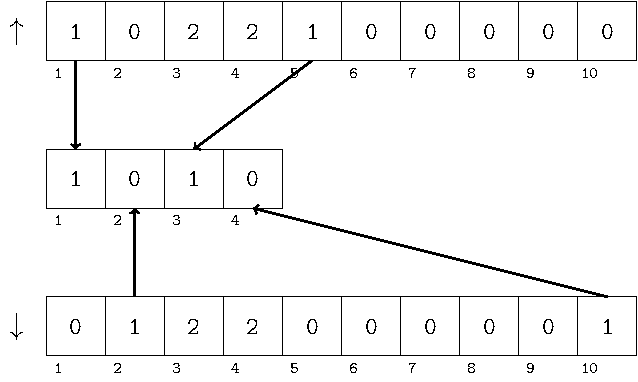
\includegraphics[width=0.9\columnwidth]{mapping}
\caption{The singly occupied orbitals are mapped contiguously in a bit string,
and the bit is one when the singly occupied orbital is of $\up$ spin.}
\label{fig:mapping}
\end{figure}


For a given {\sop}, one needs to generate all the possible spin flips that can
occur in the singly occupied molecular orbitals, keeping the numbers of $\up$
and $\dn$ electrons fixed. The generated determinants will only differ by the
singly occupied orbitals, so one first extracts the list of unoccupied molecular
orbital indices, and replaces the value of the list by 
\texttt{1} if the corresponding molecular orbital originates from the $\up$
determinant, or \texttt{0} if it originates from the $\dn$ determinant. 
Figure~\ref{fig:mapping} illustrates this mapping.

To generate all the spin flips which keeps the number of $\up$ and $\dn$
electrons constant, we need to build all the bit strings with a $n$
bits set to one and $m$ bits set to zero. 














%----------------------------------------------------------------
\section{Conclusion}
%----------------------------------------------------------------


%----------------------------------------------------------------
\begin{acknowledgments}
This work was performed using HPC resources from CALMIP (Toulouse) under
allocations 2018-0510 and 2018-18005 and from GENCI-TGCC (Grant
2018-A0040801738).
\end{acknowledgments}

%----------------------------------------------------------------

\bibliography{s2}

\end{document}
